
\chapter{The Lost Herd}

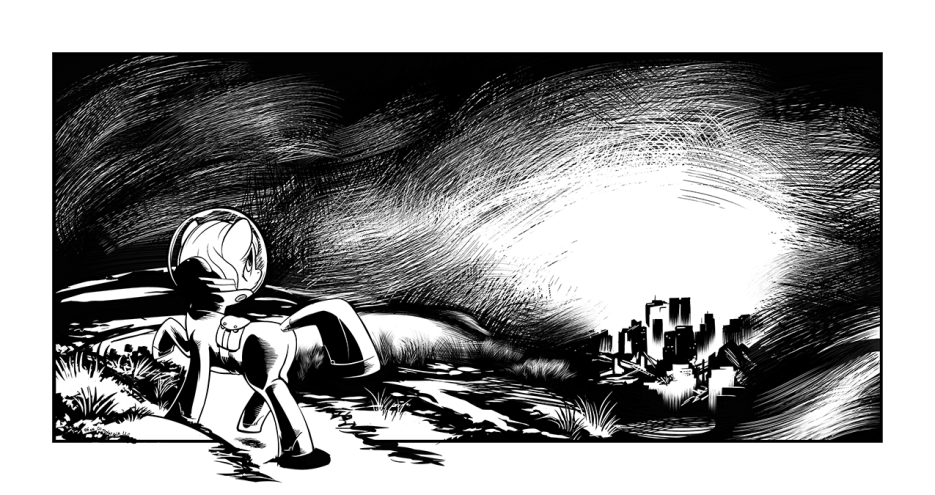
\includegraphics[width=0.9\linewidth]{image03.png}

\begin{intro}
Once upon a time, in the dying land of Equestria\dots
\end{intro}


\rtpr{``Good evening fillies and gentlecolts, this is Lonesome Pony speaking, and you're tuned to Radio 52. All the news you need to hear about Big 52 and nothing else! Well, almost nothing. In fact, it seems that now the biggest radio station in Equestria is broadcasting through all of the Wasteland. Some saint went down to Fillydelphia on behalf of DJ PON-3 and bucked the transmitter till it worked again. So hooray for those guys at Tenpony Tower, they took over the world!''}

Boisterous music played for a few seconds.

\rtpr{``Heh. That's everything from the big dogs, now back to the local news. Hey little ponies, are you afraid of ghosts? Maybe you should be. Do you remember the story of the Carnival? Don't worry if you don't. Good ol' L.P.'s going to give a quick recap for those that didn't do their homework.''}

\rtpr{``Far away on the north end of the Big 52 there lies a solitary barn. The Redtrotters call it `The Carnival.' It's a cursed relic from a long lost age, but unlike a lot of its siblings it never went to sleep. Once a year since before my grandpa could remember, a ghost would leave the building and lurk in the hills nearby, inviting everypony to its party and looking for company. When the next morning came, a foal was gone. No matter what, nopony ever returned. Approaching the Carnival was suicide thanks to the laser turrets that defended the place, but if you did succeed in getting close enough without being shot, you could hear music coming from the cursed barn, all day and all night long. A permanent party of horrors.''}

\rtpr{``Well, my little ponies, it seems that somepony just yelled 'I ain't afraid of no ghosts!', rushed inside the barn with the party in full swing and literally blew the roof off that whole place. No more foalnapping ghosts for the Redtrotters! I tried to gather some information about this benefactor, but what I got was a bit messy. Apparently, the one who did it some sort of ghost itself---a filly wearing a yellow radsuit and rising from death out of a pink cloud. Well, Yellow Ghost, nice work. One problem solved, nine-hundred-ninety-nine to go. Oh, and did I mention that this year's victim made it safely home? Celestia bless our souls! And now back to good old Pony Marcus!''}

\begin{music}
		I can see that lone star from a thousand miles away,
	
		Calling me back home, though I've ventured far away.
	
		When I see that beacon shining for me all along,
	
		It calls me to Equestria and a home!
\end{music}

\horizonline

\englishdaytimeplace{4}{00:30 A.M.}{Salt Cube Flats, Big 52 N Branch}

Puppy trotted along Route 52, heading south. The big city had grown from a silhouette on the horizon into a large, sprawling mass just a few kilometers in front of her. The foal had trotted all day long, and now the light was fading into darkness. Her eyes began to turn bright pink, shining in the night while she walked down the road. Without the daylight it was possible to see a green glow around the dome of Salt Cube City, while the bigger skyscrapers of Downtown were lit with sparse fires. The largest part of the city simply faded into the darkness of an ever-clouded night sky.

Around midnight, the filly in yellow spotted a small caravan heading in her direction from the south. There were about half a dozen ponies, and they had some sort strange two-headed cows with them. Puppy sat down in surprise, and waited for them to draw near. The caravan guards spotted the foal soon afterwards, being that she was a light source sitting by herself in the middle of the road. Needless to say, the guards were already on edge.

A large buck wearing a light combat saddle mumbled to another. ``What do you think, could it be that 'ghost' from the news?''

The leader of the guards, an earth pony mare with a big revolver, shrugged. Raising a hoof, she made the caravan stop. ``Dunno, but I'm not taking any chances. Let's move. Two on the sides, two here. I'm trying a diplomatic approach. Cover me or you can forget your pay.''

Two of the guards detached from the caravan and left the road, circling Puppysmiles, one on each side of her. Meanwhile, the leader ran ahead while the caravan with the remaining two guards kept their distance. The sight of the filly was quite an eerie one. The creepiness of the small yellow silhouette, which had a glowing pink light coming from its glassy helmet, was already a perfectly valid argument for opening fire. The leader of the guards approached the creature with caution, hoping that the other two guards were fast enough on the trigger in case of complications.

``Hi! I'm Puppysmiles!'' The foal raised a hoof, waving to the guard leader. Well, at least it didn't seem hostile.

In the Wasteland Survival Guide, there's a sentence that dwarfs all others when it comes to the sheer number of iterations: \emph{better safe than sorry.} Not seeming hostile didn't mean it was safe. ``Okay, now don't move, and tell me what you are and why I shouldn't transform you into fertilizer.''

Puppy giggled. Fancy words always made her giggle. ``Tee-hee, pretty pony is funny! I'm not Forty Liza, I'm Puppysmiles! What's your name?''

The guard leader hesitated for a moment. Was this foal simply retarded, or was it all part of some well-planned trap? The whole situation just smelled wrong. ``Yeah, I'm Solid Slug. Are you alone?'' Without waiting for an answer, the guard gestured to the two on her sides to check the surrounding area.

``Nopey mopey, I'm with Mister Voice! He's super smart or super stoopid, it depends. But for sure, he knows where my mom is!''

``And where is this `Mister Voice' now?''

``Inside the space suit! See all the lights and the pretty dots? He makes them appear!'' Okay, there was a nine out of ten chance that she was just a retard.

Solid Slug took a better look at the suit's helmet, trying to ignore Puppy's brightly shining eyes. There was an active HUD, quite similar to the one used in some models of battle saddles. Upon closer examination, the harness seemed like a very expensive piece of equipment. Solid wondered how a foal could ever find something like that, but the pink light emanating from the suit gave her the feeling that there was more to the situation. Solid Slug had been in the business for a whole lot longer than most caravan guards, and had picked up more than a thing or two about the Wasteland in all that time.

``Say, are you from Canterlot by any chance?''

``Yush! My house is, ah, was just under the mountain in Clover Leaf Terrace, but the other day it went down, so now I'm looking for my mom. She wasn't at the old barn, but Mister Voice says that there is another place in that big town so I'm going there now!'' Puppy pointed a hoof somewhere southward.

Solid Slug nodded a couple of times while listening, raised a hoof and gestured to the caravan. After some preparations the carts started moving again. ``Wow, you chat a lot, don't you? Lonesome Pony was speaking about your exploit at the Carnival.''

``My what? You mean the old barn? I didn't explode there, it was the barn that exploded, silly filly.'' Puppysmiles giggled. ``That Pinkbot was totally a baked bad! At first it was really creepy, but I'm a brave pony!''

Solid Slug scratched her head, trying futilely to follow Puppy's chattering. ``Uh, yeah, that's great. I'd stay here and chat for ages but we have to keep moving. If you're going to Salt Cube City, the ghoul community is at the Dome. I think they call it the Glow. Don't wander too much in Downtown, they don't like your kind. Oh, and, well, good luck, little ghost.'' When the caravan arrived the other ponies of the group sneaked curious looks at Puppy, but Solid Slug whispered to a purple unicorn with a red mane, and they simply kept moving. The filly in yellow stared with amazement at the brahmins and waved a hoof to the pretty ponies as they disappeared into the night. Once she was on her own again the foal trotted away, heading south along the Route.


\horizonline

\englishdaytimeplace{4}{11:30 A.M.}{Downtown, Salt Cube City}

The gate was a simple barricade built from sandbags and salvaged metal plates. On a wooden platform, a pony with metal barding operated a chaingun, while two other guards checked every pony that wanted to get into Salt Cube City. One last unicorn wearing an officer's uniform sat inside a small metal structure making notes in a register.

It was almost noon, but the traffic on the north end of downtown was as dead as the Wasteland. This time Puppysmiles was ready. She had that metal thing with the painted apple and showed it to the guards. One of the armored ponies approached her while the others kept their weapons ready.

``Let's see. Yes, this is a valid pass. Now, what's your name and business here?''

``I'm Puppysmiles! What's your name mister pretty pony?''

The guard raised the visor of his helmet, giving Puppy an annoyed look. ``Corporal Farsight. Now, what's your business in Salt Cube City, kid?''

``Oh, I know this one! I'm looking for my mom! She's somewhere in that direction!'' Puppy pointed her hoof toward a cluster of ruined buildings and the guard sighed.

``Very well, I guess that's enough. Just another question---why are you wearing a full environmental suit?''

``Oh, this one? I'm stuck inside it, but that's okay because Mister Voice lives in the space suit too and he's helping me with my mission.'' She lowered her voice, whispering to Farsight, ``He's not very good with that, but don't tell him. He's quite grumpy.''

The guard lowered his visor again and shrugged. ``As long as you're not going to blow a megaspell in Downtown, you can dress as you like. Welcome to Salt Cube City, kid.'' Puppy trotted beyond the roadblock, but Farsight called her back one last time. ``Oh, and don't go anywhere near the Dome. There are feral ghouls in the area, and it's heavily irradiated.''

``Okie dokie lokie! Bye bye mister guard Farsight!'' Puppy trotted merrily toward the big skyscrapers at the bottom of the boulevard, although the pink arrow pointed in a different direction.

Downtown was a typical trade hub along the Big 52. There were guards that kept ponies from killing each other and a couple dozen tents with signs of the different trading companies operating in the area, like the Water Herders or the Bullet Gallopers. There were even freelance traders and some trading posts from the nearest tribes. The open market was placed in the streets, but the real Downtown consisted of the four skyscrapers that still stood in the middle of the settlement. Salt Cube City had been the target of a single megaspell during the war, and the missile vector that should have delivered it malfunctioned. The warhead hit the Salt Cube Dome in the city periphery, piercing the roof and exploding at ground level. The massive structure of the Dome had shielded the surrounding area from the worst effects of the direct hit, but not from the fallout. During the successive two centuries, the most weathered buildings surrendered one by one to the ravages of time, but the four biggest and least-damaged skyscrapers survived and still stood in the middle of the city.

The four towers were the symbols of power in Salt Cube City. Two of them were each the main hub of a trading company, while the third was the headquarters of the Hired Hooves, a powerful mercenary company. The last building was the smallest one and housed the White Apples, the original tribe that inhabited the city. They were formally the real proprietors of the whole town and got a share of all the commerce going on in the place. The White Apples were also the main breeding ground for the Hired Hooves, mostly consisting of the families of ponies that worked for the mercenary company.

Puppy stood in front of a small tent marked with a red splash, the symbol of the Redtrotters. The shop sported a vast array of melee weapons and light armor on the shelves. A mare with an old cowboy hat was sitting on an ammunition box just in the middle of the exhibition.

``Hey, nice dress, little one. Say, are you from the north?'' The mare smiled at Puppy and lifted her hat with a hoof, revealing a horn on her forehead. The cutie mark on her flank depicted a basket ball.

``Hi! I'm Puppysmiles!'' She waved a hoof and trotted toward the mare. ``I'm from there.'' Puppy pointed at the street outside the tent.

``I'm Play Maker. I think that Lonesome Pony mentioned something about you last night.''

``Uhm, you mean the chatty pony on the music channel?'' Puppy scratched her helmet with a thoughtful expression. ``Last time he was speaking of the importance of drinking pure water.''

``No, no, I mean the news about the Yellow Ghost. Uh, maybe there's more than just one pony wearing a radsuit around. Anyhow, what do you need?''

Puppysmiles frowned. ``Why is everypony calling me a ghost?''

Play Maker smiled. ``So it's you after all, I knew it!'' The unicorn tapped her chin for a moment. ``Say, aren't you a bit too young to destroy a cursed barn? Actually, aren't you a bit too young to go around on your own? Are you a Crusader?''

``Nopey mopey. I'm looking for my mom, and I'm not alone! I have Mister Voice with me.''

``Your mom? Maybe I can help you: a lot of ponies visit Downtown every day. What's your mom's name? What's her cutie mark?''

Puppy smiled widely. ``Oh, her name is Rainy Days, she's purple and has an orange mane and her cutie mark is a cloud with raindrops! Have you seen her? Mister Voice says that she's somewhere in this place! That way!'' Puppy pointed her hoof again in the direction of some destroyed buildings.

Play Maker shook her head. ``I'm sorry, kid. Can't remember a pony with that palette or cutie mark, and the name doesn't ring a bell.'' She looked in the direction that Puppy was pointing and frowned. ``That way, you say? That can't be good. That's the radioactive area. The only standing building in that direction is the Dome, and trust me, you don't want to go anywhere near the Dome.''

``The Dome? What's that?''

``It's a place filled with feral ghouls and other horrors. It's highly radioactive, but maybe that's not a problem since you're wearing a radsuit. The real problem is the inhabitants: a small community of fanatical religious ghouls live there, but they're on the brink of madness. In fact, some of their 'siblings' went mad and attacked the caravans heading here. There's quite a situation now, and the White Apples are looking for a way to get rid of those rot-heads. They blast any ghoul that shows his face outside, but they can't go in and finish the job. The whole place is a deathtrap if you're not immune to radiation, so they reached a stalemate.''

Puppysmiles frowned. ``What's a ghoul?''

``You're kidding me! You don't know what a ghoul is?'' Play Maker stared at the blank expression on Puppy's face and sighed. ``No, you're not kidding.'' She shook her head. ``A ghoul is a pony that was poisoned by radiation a long time ago, when the megaspells hit. Instead of dying they were transformed into---I'm not sure what they are. The living dead? Maybe some sort of zombie? Anyhow, many of them went crazy because of that mutation and became feral ghouls---aggressive creatures that attack and try to eat everypony they see. Others retained their sanity and became immortal, but were disfigured by the mutation. Their manes fell out, their hides burned away, and their flesh began to blister and rot. Every ghoul looks like a decomposing corpse, but somehow they remain alive. The problem is that sooner or later every ghoul goes `boing' in the head and swaps their current diet for a meatier one.''

Puppy frowned. The unicorn could see fear and realization in her eyes. ``Miss Play Maker? Um, if my mom is really where Mister Voice says, will she be okay?''

``I---'' She lowered her hat, hiding her eyes from Puppy. ``I don't know, little ghost, but the Dome is a dangerous place. I hope you're not going there after what I told you.''

Puppy stood on her hooves with renewed determination in her eyes. ``I have to go! My mom could be there, and she could be in danger!''

Play Maker immediately realized that she'd never be able to talk her out of this suicide mission. ``You're not family, so I can't tell you what to do and what not to, but please listen to my advice. Go to that tower, the one with the big white apple on the sign. Tell the pony at the entrance that you want to enroll for a scout mission into the Dome. They'll give you some equipment and maybe a weapon. You have a radsuit, and they're so desperate that they'll accept anypony that they think could at least stand a chance.''

Puppy smiled. ``Okie dokie lokie! Hang on, Mom, I'm coming to rescue you!'' The foal galloped out of the tent and eagerly rushed to White Apple Tower.


\horizonline

\englishdaytimeplace{4}{2:00 P.M.}{Salt Cube Dome, Salt Cube City}

{\mt ``Warning. Mild radiation detected. Threat level: negligible.''}

The Dome was a humongous elliptical structure that had once served as an expo center where a large number of events could be hosted at the same time. A gigantic, globular roof once covered the building, but now it was almost completely destroyed, leaving only the external walls still adorned with columns and arches that made the structure vaguely resemble an oversized coliseum.

A boulevard headed right to the main entrance of the Dome, a monumental arch that led into a hall where the huge remains of a marble statue littered a floor that was once made of polished stone tiles. Now, it was mostly a carpet of rubble. Puppy stood in front of the archway, looking at the pink arrow on the compass.

``Okie dokie Mister Voice, what are we doing now exactly?''

{\mt ``Ministry of Morale hub reached. Primary objective attained.''}

``Yes, I know that we are here. I'm asking what's next. What are we supposed to do here?''

{\mt ``Secondary objective: investigate the ghouls and/or get rid of them. Warning. Mild radiation detected. Threat level: negligible.''}

``So, we find these ghouls, ask them where is Mom and then we try to make them go away?''

{\mt ``Affirmative. This is one possible approach.''}

``Great, I love having a plan. Let's do it.'' Puppy stepped into the hall and yelled, ``HEY, GHOULIE PONIES!'' It echoed several times into the large structure. She didn't seem to get any answer, so the filly in yellow trotted toward a large staircase at the bottom of the entrance hall.

{\mt ``Warning. Heavy radiation detected. Threat level: negligible.''}

``Hey, I think I've seen somepony moving behind that statue! Hey you, wait!'' Puppy galloped in the direction of a shadow that was hiding behind the pedestal of another broken marble monument. As the foal reached the hiding pony, she slowed to a trot and called out to him or her. ``Hi, I'm Puppysmiles! Have you seen my‒''

That pony! It was him---Count Horse Tile! He was right in front of her, even uglier than she could remember and somehow a lot creepier.

{\mt ``Warning. Hostile detected. Feral Ghoul. Distance: two meters. Threat level: low.'' The creature was looking at Puppy's face, drooling a yellowish goo from its mouth. It seemed oddly uncertain about its next move.}

Puppy stepped back, terrified by the macabre sight. ``W-why are you still coming after me? Leave me be! Go away!''

The creature growled and lowered its head, so Puppy turned on herself and galloped away as fast as she could.

Alas, it wasn't fast enough.

The feral creature jumped on her, foaming and biting, aiming for Puppy's head. The helmet was designed to endure punishment, so the first assault of the raging beast simply hurt Puppy's innocence. The sight and sound of a mouthful of rotting, jagged teeth scraping against her helmet was enough to paralyze her with fear.

``EEEEEEEEEEEK!'' Puppy reacted on pure instinct. She tried bucking the ghoul away, but it was a lot heavier than she was, and it pinned her on the ground with its weight. ``Rock! ROCK! NOW!'' She didn't stop screaming as she grabbed \emph{The Rock Of Destiny} with both hooves and started hitting the monster repeatedly. ``Stop moving! STOP MOVING NOW!''

A couple of minutes later, Puppy was still beating the brown slimy pulp that was once a pony's head. The scratches on her helmet and some minor bruises on the fabric were already gone thanks to the self-repair spells built into the suit. Slowly, the beating simmered down until it stopped completely. The ghoul was positively immobile and Puppy needed to catch her breath. It had been terrible, but at last the dark shadow of Count Horse Tile was gone! No more hiding or running away. The monster was stopped once and for all, his reign of terror extinguished! At last Puppy felt relieved, until she raised her eyes from the dead ghoul.

And finally noticed the three other ghouls that were looking at her with empty eyes and drooling mouths.

{\mt ``Warning. Three hostiles incoming. Nearest target: twelve meters.''}

``Hey, Mister Voice. What is a miss under---uh---static?''

{\mt ``Misunderstanding. The act of giving the wrong meaning to a word or sentence, creating confusion. The more you know!''}

Puppy nodded slowly while the three ghouls looked in her direction from the end of the hall. ``Good. What is exactly a Horse Tile Count?''

{\mt ``Hostile count. Number of enemies or ill-intentioned creatures in sensor range. Actual hostile count: three. Feral ghouls. Threat level: moderate.''}

Puppy sighed, threw \emph{The Rock Of Destiny} at the ghouls, and charged. The ghouls did the same thing from the other end of the hall.


\horizonline

\englishdaytimeplace{4}{2:30 P.M.}{Salt Cube Dome, Salt Cube City}

{\mt ``Warning. Several breaches in the containment suit. Warning. Littlehorn Agent detected. Warning. Compass malfunctioning. Warning. Inventory management spell temporary offline. Warning. Energy crystal cells damaged. Emergency cells on 29.06\%. Warning. Deadly radiation level detected. Threat level: negligible. Subject deceased, condition stable. All clear.''}

Puppy stood in the middle of a scene of mayhem, decorated with goo and rotten flesh. The bodies of three ghouls lay scattered on the ground with their heads missing. The whole fight had taken a while and been very messy, since the ghouls kept regenerating because of the radiation in the area. However, Puppy had also been regenerating because of the Pink Agent and her radsuit's enchantments. In the end, the foal's dedication at aiming only for their heads won out over the brainless biting and bucking of the ghoul trio, but in the process she had been beaten like a bucking bag. Her flanks had been half eaten and a thin pink cloud invaded the area.

``Hey, Mister Voice? Are you sure that Mom is in this place?''

{\mt ``Affirmative. Actual position: Ministry of Morale structure ID 00201--Salt Cube Dome.''}

``Okie\dots dokie\dots lokie\dots'' Puppy stopped listening at affirmative and fell to the ground, exhausted from the fight. ``Because the only thing I want to do now is cry.''

A couple of figures appeared from another entrance of the hall. They seemed to whisper to each other before one of them took a hunting rifle while the other moved cautiously toward the filly in yellow. Puppy reached out with her hoof for \emph{The Rock of Destiny} in front of her and grabbed it, but her eyes were so tired. She just wanted to lie down a little more. ``Please, go away. Please,'' she whimpered, ``stop being mean. I'll behave.''

The nearest pony now was close enough to let Puppy take a good look at it. It was another ghoul, but somehow different from the others. This one was wearing a uniform similar to the one of the mare that gave her the suit. Moreover, it didn't drool, had some intelligence in its eyes, and last but not least, it spoke.

``Hey, are you okay little one? This place is very dangerous.'' The pony sounded like chalk screeching on a blackboard, but somehow Puppy felt like it was a mare's voice. ``Hey, Soft Air! We have to take this foal out from the radioactive zone before she dies! Do we have any Rad-X or some RadAway?''

``I don't think so. Stay out from the pink cloud, it seems awfully familiar. I'm almost positive it's dangerous.''

The scouting pony abruptly stopped before getting too near to Puppy and tilted her head. ``Oh, so it's not just my bad eye?'' The ghoul trotted around the pink cloud that was quickly dissipating, as if the suit were drawing it back inside itself in the process of self repairing.

{\mt ``Containment restored. Warning. Critical level of radiation detected. Threat level: negligible.''}

Puppy slowly rose to her hooves while the ghoul mare drew near and the other kept his weapon ready. The filly had to try something diplomatic. ``I, uh, hope that those ugly ponies weren't your friends?''

``The word you're looking for is ghouls, little one. And yes, there was a time when they were our friends, but I guess that right now you did them a favor. So, no bad blood.'' The ghoul mare stopped in front of Puppysmiles and took a look inside her helmet. The face of the filly was annoyingly well conserved, not showing scars or signs of deterioration, but the pink flames in her eyes, burning bright with the radiation of the place, spoke volumes about her nature. ``You are quite a strange ghoul. I'm Peach Blossom, what's your name?''

``Uhm, oh, yeah, I'm Puppysmiles. I'm looking for my mom, she's supposed to be somewhere in this place but all I found were these ugly ponies.''

Peach waved a hoof, calling her companion. ``Soft Air, stop being paranoid and come here!'' She went back to speaking with the foal in yellow. ``Could you please stop calling us ugly and just say ghouls? Anyhow, if your mother is here she has to be a ghoul too, otherwise she is going to be super slim. What's your mother's name?''

``I know this one! Her name is Rainy Days and she's super cool! Have you seen her?''

The buck coming near overheard the conversation. ``Rainy Days, Rainy Days\dots That name sounds familiar. If you give me a second or two to think about it I might remember something.''

Puppy looked amazedly at Soft Air. ``Really? Please please please where is she?''

``Hey, wait, I told you I can't remember her very well! My memory is not as good as it used to be. Anyhow, if you don't want to meet other ferals we should move. Let's go to the Glow.''

Peach Blossom nodded. ``Yes, let's get back, after all we found what we were looking for. Anyhow, Puppy, where are you from?''

``Canterlot!'' Puppy smiled with pride. Canterlot was the best city ever, why not be proud of it?

Both ghouls frowned, Peach looked away while Soft Air sighed. ``Oh, so you are one of those.'' Peach muttered to herself. ``War sucks.''


\horizonline

\englishdaytimeplace{4}{3:00 P.M.}{The Glow, Salt Cube City}

The Glow was mostly a small circle of tents pitched in the central hall of the Dome. The roof was missing and large metallic debris littered the ground. The tents were all sporting a symbol of three pink butterflies on a yellow background, and were large and sturdy, being made of a tough material that was built to last. They had survived for more than two centuries.

Quite obviously the Glow wasn't called as such because of the tents, nor for the ghouls. It was the twelve meter tall salt cube glowing in a blueish-green light that earned the Glow its name.

{\mt ``Warning. Radiation level off the scale. Sensor emergency shutdown activated in order to prevent irreversible damage. Threat level: negligible.'' The HUD of the helmet disappeared. Puppy frowned for a single moment, then shrugged. Maybe even Mister Voice needed a little sleep sometimes.}

The cube was drawing all of Puppy's attention at the moment. It was shiny and glassy and super nice. The foal wondered if she could have some little shining cubes to keep in her bedroom. This could get rid of that bad scary monster that lived under her bed. For a moment she missed her home and felt like crying, but she was a filly on a mission, and she didn't have time for these things, so instead she asked, ``What's that pretty shiny cube? Can I have a shiny cube too? Please? Puppy please?''

Soft Air chuckled. ``I don't think so, Puppy, but I could have something nice for you if you will be a good pony. Deal?''

Puppy started jumping all around. ``A present? For me? Gimme gimme gimme!''

``Now, now, I told you to behave, right? First of all we are going to have a little chat with Sand Box, then we'll try to find out about Mrs.~Rainy Days.''

Puppy stopped jumping and began to trot alongside Soft Air and Peach Blossom. ``You know? Even if you're pretty ugly you are funny and nice ponies.''

Peach deadpanned. ``Well, thank you, miss monster. Anyhow, there he is, Sand Box, the leader of the camp.'' Another ghoul was looking at a block of paper, reading it and scratching his head seemingly in confusion. ``Even if he seems elsewhere at times, he's smarter than the average scientist. Hey, boss, we got a visitor.''

The leader of the ghouls was wearing an old lab coat and a pair of glasses, and seemed quite alarmed from the look he was giving the papers in front of him. The ghoul replied without even looking at Puppy. ``Yes, great, give him the usual speech and warn him against Downtown. Excuse me, but I'm trying to avoid a cascade.''

Puppysmiles giggled and trotted up to him, trying to look at his face. ``Tee-hee, ugly pony says fancy words! Hi, I'm Puppysmiles, but you can call me Puppy! Have you seen my mom?''

Peach tried to stop the foal but it was already too late. She opened her mouth to speak, but was interrupted by the reaction of her leader. Sand Box adjusted his glasses and studied Puppysmiles for a moment. ``Luna buck me if I thought I'd see another functioning Mark VI. That was a hay of a failure, wasn't it?''

Both Peach and Air tilted their heads, staring in puzzlement at Sand Box as he continued. ``They were designed to keep foals safe from the worst effects of a fallout, loaded with all the best medical talismans and up-to-date logical spells that in some cases were even more advanced than the ones used by Stable-Tec in its PipBucks.'' He shook his head, his expression turning sad. ``What we didn't expect was the reaction of all this technology and magic in case of a Pink Agent attack. The suits had enough medical supplies and healing power in their talismans to mitigate the first effects of the gas, creating the perfect conditions for a uh, merging process.'' The scientist turned toward the other two ghouls. ``Have you ever heard of the Ghost Herd?'' Both ponies shook their heads. Sand Box put a hoof around Puppy's neck, making her stand next to him.

``It was about a month past the day the Goddesses fell. A small herd of little ponies wearing yellow suits, just like this one, left Canterlot. Most of them lost their minds because of the mutation, the others had simply no clue about what was going on. They were ghosts indeed\dots Obsessed with the loss of their parents, and clueless about what happened, they wandered together mostly because everypony else in those days was dead. The herd came here, heading south. They met some survivors on their path, but the crazed ones simply slaughtered any living thing that they met. The others, well, they were afraid of being alone and followed the herd.''

Peach stepped back. ``She doesn't seem that dangerous to me.''

Sand Box chuckled and kept narrating his tale. ``They are mostly immortal like us ghouls, but they rise from their own dust unless you tear their bodies apart, like Canterlot ghouls. Even worse, the MK VI has a very advanced self-repairing spell that lets them recover even from some amputations and such. They are quite the little yellow devils.''

Soft Air tapped his chin. ``But if they were so invincible, where are they now?''

``I have no idea. Most of them were taken down, at last. A decapitation combined with the destruction of the main spell matrix and the backup system should do the trick, but it's not that easy if you don't know what you're doing. Anyhow, at some point they left, disappeared and were never heard from again. The whole thing lasted a couple of months at most. You had to be there to remember them, but it was quite a disheartening sight. All those foals left alone and cursed in a dying world. Poor things.''

Sand Box patted Puppy on her helmet. She listened to the whole story trying to follow it, but she seemed a bit confused. ``I don't like this story, it makes me sad.'' Sand Box simply sighed and kept his hoof around Puppy's neck.

``Don't worry, little one. It's just an old ghost story, don't let old mare tales sap your enthusiasm. I think I have a Pinkie Pie plushie somewhere. Let's do this: just tell me why you are here and I'll give it to you, yes?''

A large grin appeared on Puppy's face, the boring story of the ghost herd already forgotten in favor of a way more interesting new toy. ``Sure! I'm looking for my mom! Her name is Rainy Days, and she is the best pony ever!'' Puppy seemed to remember something else. ``Oh, right! And I'm here to tell the ghouls to go away and never come back! Have you seen any ghouls around, Mister Ugly Pony Boss?''

Peach Blossom facehoofed.

~\vfill

\begin{engnote}
	Level up! (2)
	
	New perk added: Little Leaguer - You gain a +5\% in throwing, melee and unarmed combat.
\end{engnote}


